\documentclass{beamer}
\usepackage{presentation}

\begin{document}

\frame{\titlepage}

\begin{frame}
  \frametitle{Introduction}
  \begin{quote}{}
    \input{build/goal_statement_md}
  \end{quote}

  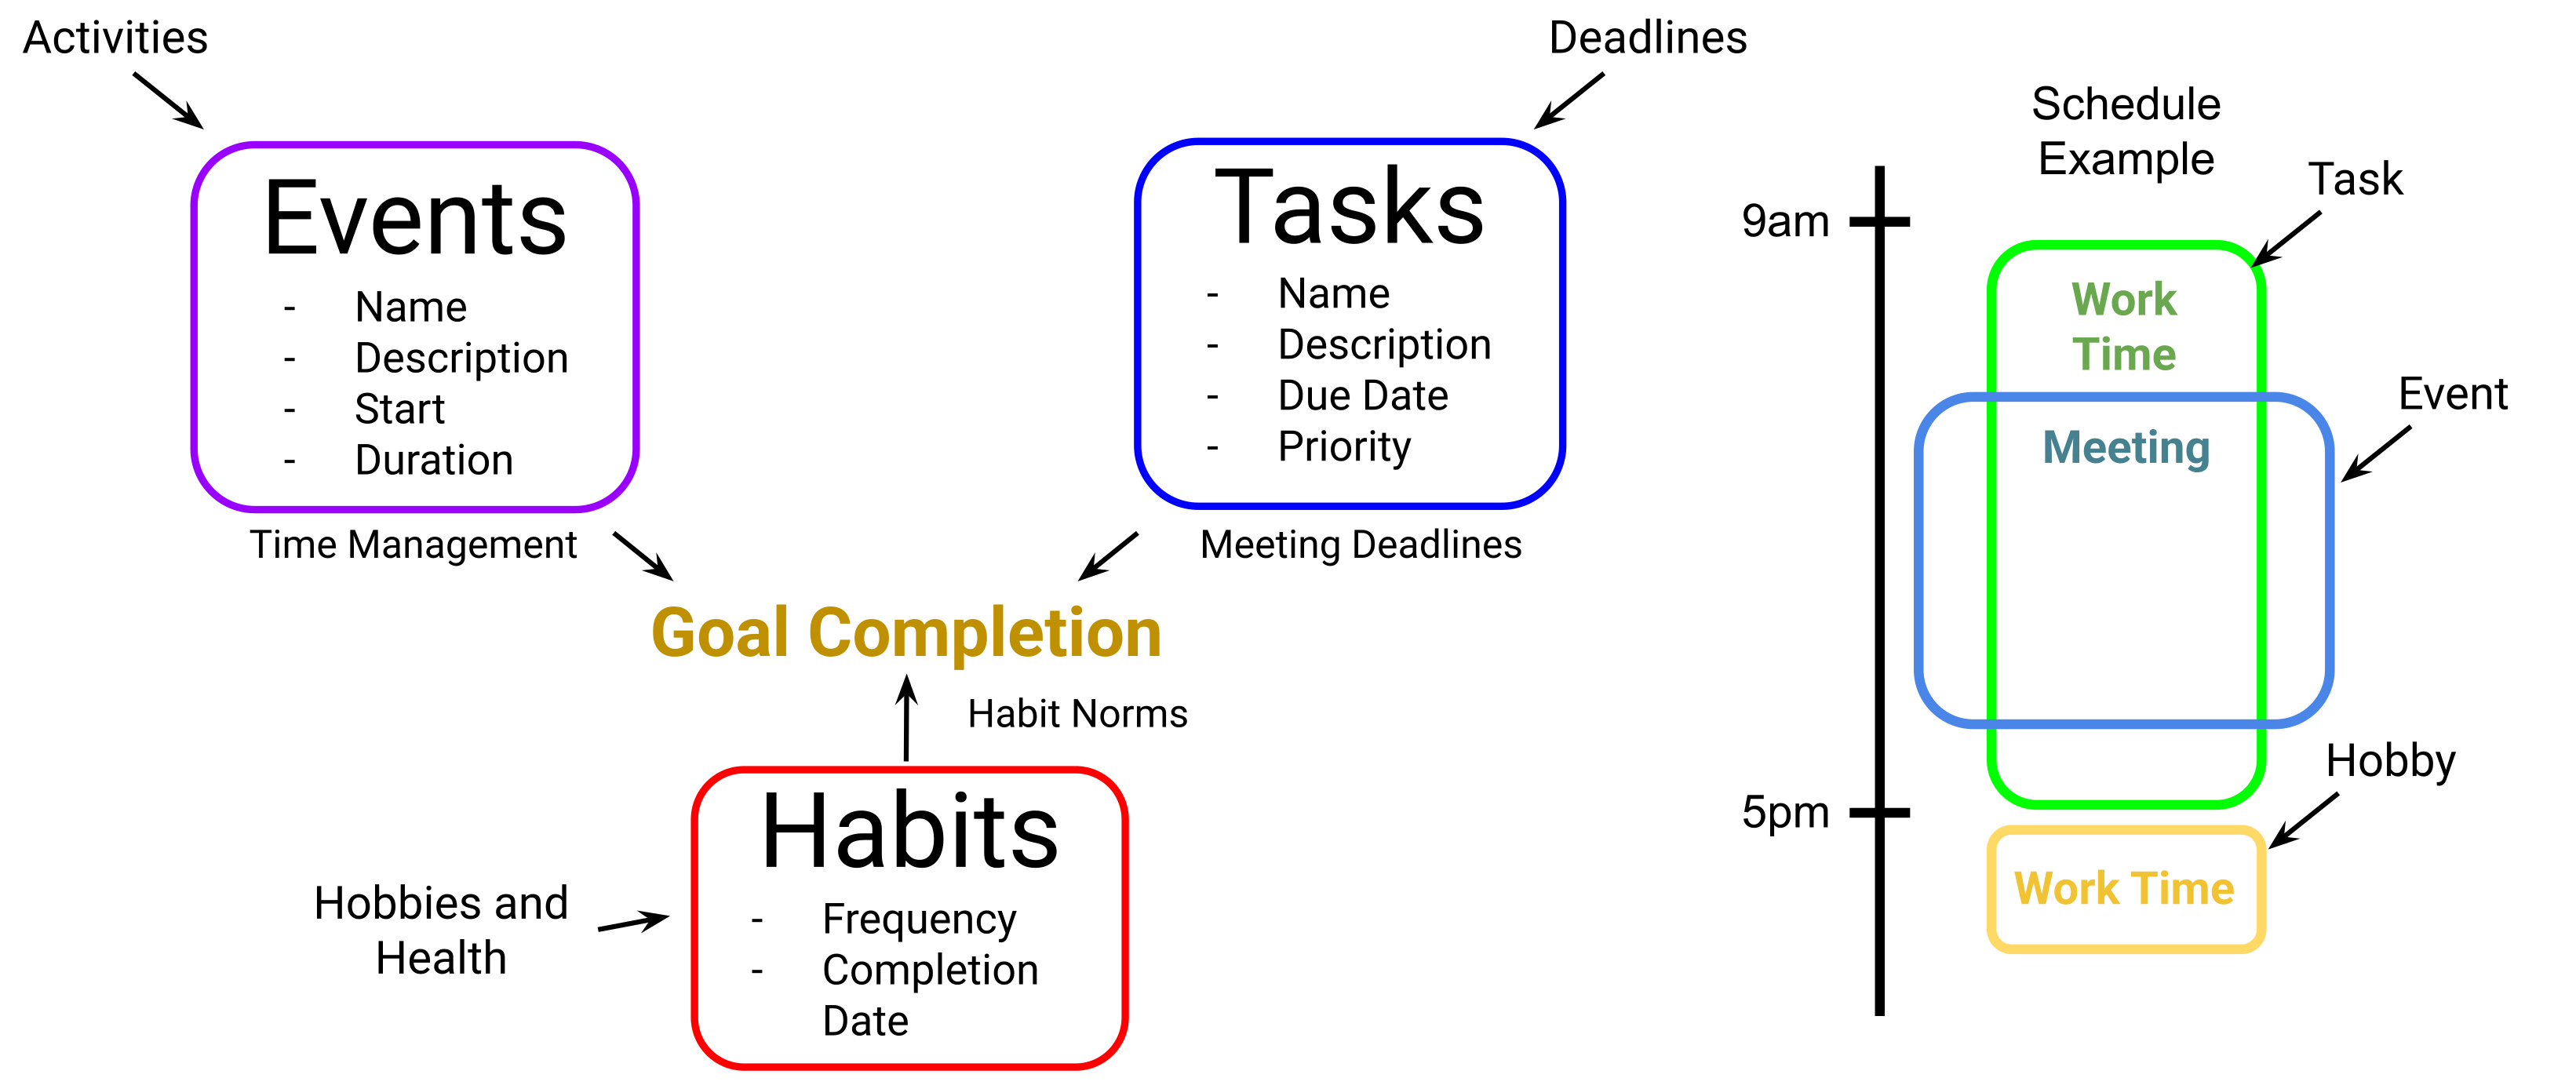
\includegraphics[width=\textwidth]{images/goal_completion.png}
\end{frame}

\begin{frame}
  \frametitle{Prototyped elements of design}
    %TODO TABLE OF ALL MANUFACTURED PRODUCT FEATURES, COLOR WHICH ONES WE DID IN PROTOTYPE
\end{frame}

\begin{frame}
  \frametitle{Biggest Roadblock: Memory usage}

  The prototype design ran into memory availability issues
  \begin{itemize}
    \item 188 kB of static memory (58.4\% of available memory)
    \begin{itemize}
      \item 66 kB used by graphics
      \item 60 kB used by neworking
      \item 133 kB left for dynamic memory
    \end{itemize}
    \item Different features
    \begin{itemize}
      \item BLE for Wifi info
      \item Persistent connection
    \end{itemize}
  \end{itemize}
  There are better boards that could have been used for the prototype

  \note[item]{GPU option: If we utilized dual cpus for the graphical display , display would be faster}
  \note[item]{LVGL already supports custom external gpu rendering}
  \note[item]{With more memory and parallel processing, current approach should
  be more performant}
  \note[item]{This taught us our hardware requirements for the manufactured product}

\end{frame}

\begin{frame}
  \frametitle{Wi-Fi and MQTT}

  \begin{itemize}
    \item Wi-Fi provisioning + connection + MQTT = 100 kB (static \& dynamic)
    \item No memory = no persistent session = no stored messages
    \item User makes change $\rightarrow$ need to send entire backup
  \end{itemize}

  An HTTP server that responds to "changes since X" may be a better approach.

  \note[item]{persistent sessions store non-ack'd qos = 1 messages}
  \note[item]{after a reconnect, non-ack'd items are re-sent}
  \note[item]{instead of connecting and having a worker thread, the prototype
  connects, spends 5s, then disconnects, ending the session}
  \note[item]{Final product asks for the entire thing on power-on, then react to any
  new messages during the persistent connection.}
\end{frame}
\begin{frame}
    
  \frametitle{What did we learn from the prototype?}

  \begin{columns}
    \column{0.5\textwidth}
    What worked:
    \begin{itemize}
      \item SQLite3
      \item Persistence
      \item Web server
      \item Wi-Fi provisioning
    \end{itemize}

    \column{0.5\textwidth}
    What is improved in the manufactured product:
    \begin{itemize}
      \item MQTT
      \item Memory usage
      \item SoC specs
      \item Device authentication
      \item Additional features
      \item Screen size and touch
      \item Haptics and audio 
    \end{itemize}
  \end{columns}

  \note[item]{MQTT: no persistent connection --- no message \textit{queue}}
  \note[item]{ESP32-C3: RISC-V SoCs do not support memory expansion}
  \note[item]{Discuss potential alternatives: ESP32-S3, Teensy 4.1, STM32H7 line, Pi Zero 2W}
  \note[item]{Components: add aptics, audio, improve screen and touch}
  \note[item]{Additional features: time blocks, event organization}

\end{frame}

\begin{frame}
  \frametitle{Server Architecture}

  \begin{center}
    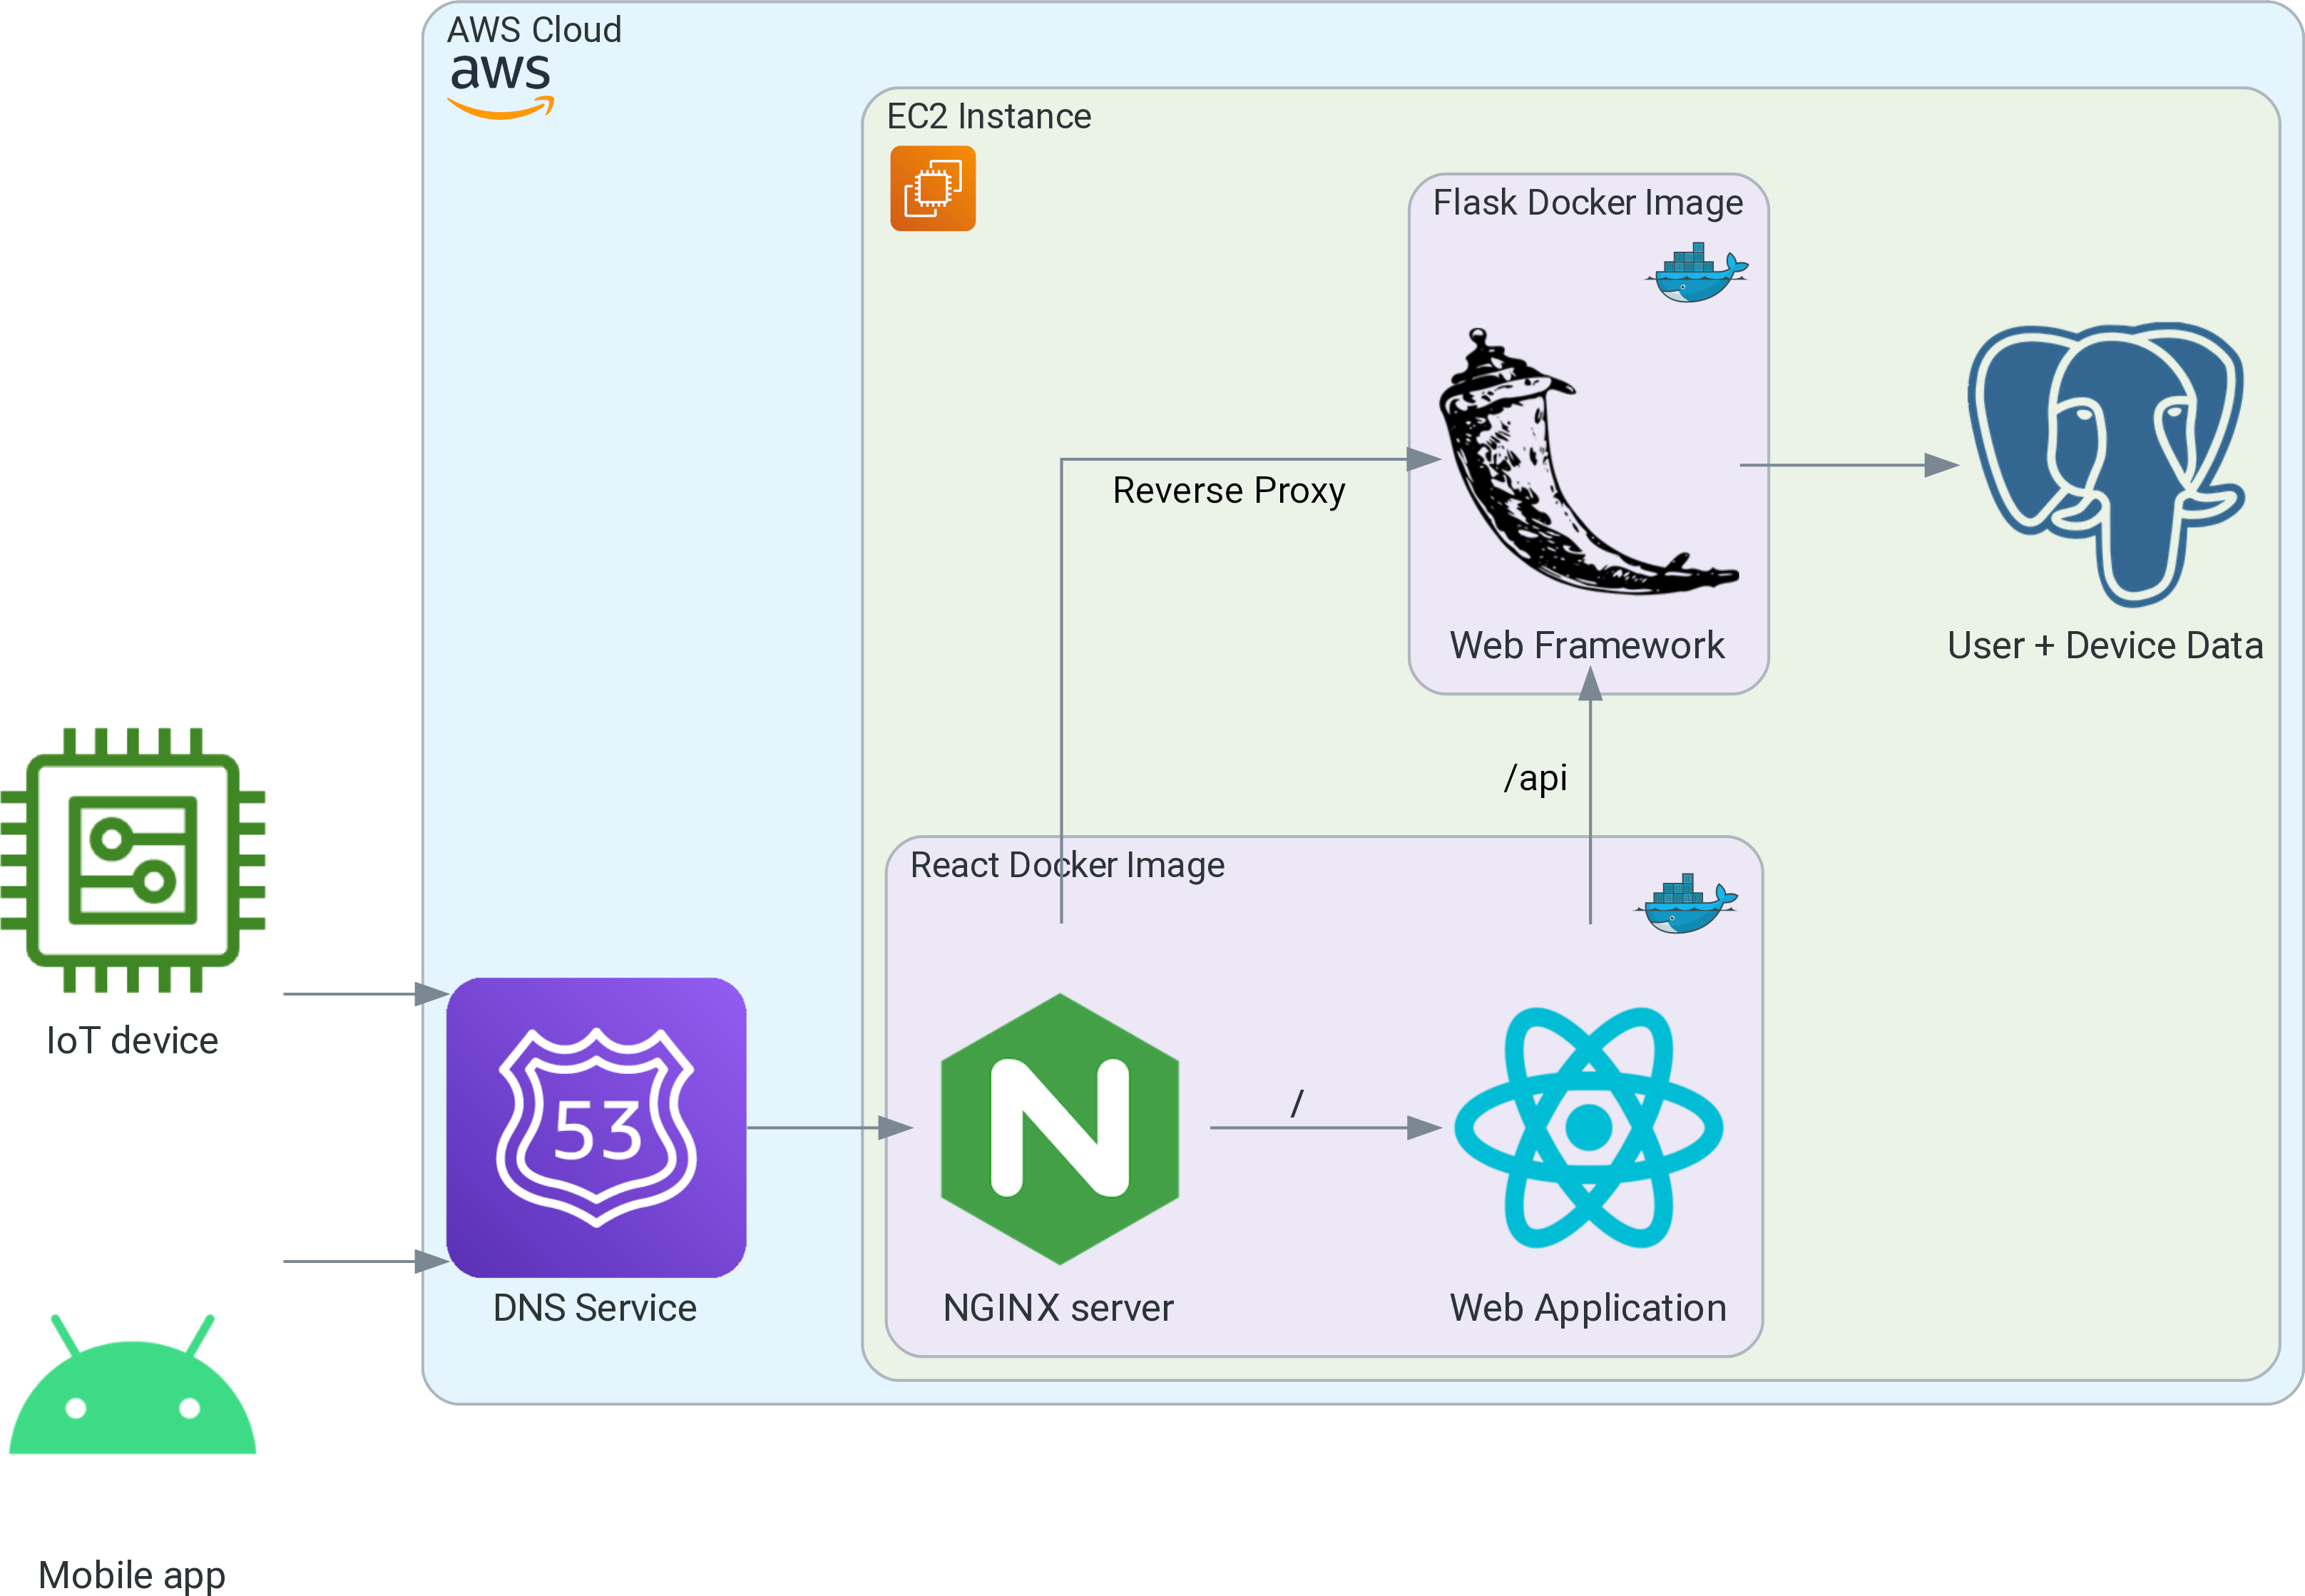
\includegraphics[width = 0.9 \textwidth]{data_flow.png}
  \end{center}

  \note[item]{React web app and the device will make requests to "/api" to
  interact with the server data}
  \note[item]{Both user and device will interact with the api after ensuring
  they have an un-expired jwt}
  \note[item]{With device jwt, we should have better security and a proper
  device authentication process}

\end{frame}

\begin{frame}
  \frametitle{Tests}
 %tests we can and cant do 
\end{frame}

\begin{frame}
  \frametitle{Test Results}
 %results of tests we did 
\end{frame}

\begin{frame}
  \frametitle{Initial goal}

  \input{build/design_objective_table_md}

  \begin{center}
    Did we succeed?
  \end{center}

  \note[item]{No to sync time}
  \note[item]{Battery seems feasible}
\end{frame}

\begin{frame}
  \frametitle{Finalized Specs}
    %TODO NEW DESIGN OBJECTIVE TABLE WITH WHAT THE MANUFACTURED PRODUCT ACTUALLY WILL HAVE

\end{frame}

\begin{frame}
  \frametitle{Final Manufactured Product}

  \begin{center}
    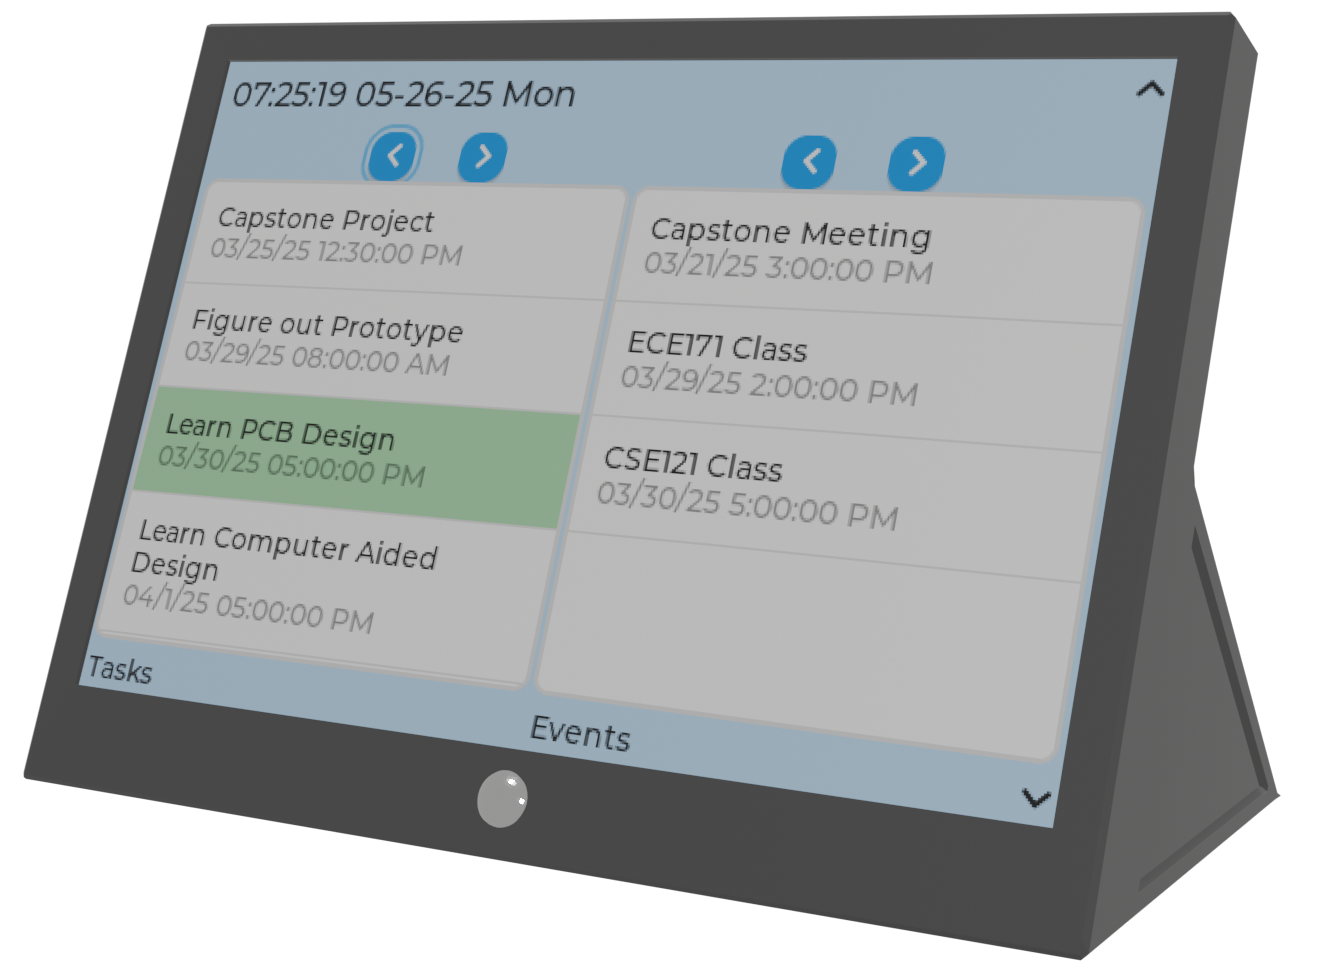
\includegraphics[width =\textwidth]{schedule_companion_render.png}
  \end{center}
  %TALK ABOUT DESIGN CHOICES FOR NOT KICK STAND, TALK ABOUT REPAIRABILITY

\end{frame}


\end{document}
